\subsection{OpcuaServer}
Die Klasse \eigenName{OpcuaServer} (\refFig{fig:backend:classDiag:OpcuaServer}) implementiert einen \ac{opcua} Server, um die \emph{DataNodes} des \ac{scada} Systems einer Menge an \acp{plc} zugänglich zu machen.
Sie bedient sich dabei der C Bibliothek \eigenName{open62541} \citep{open62541:lib}.
Der Entscheidung, diese Bibliothek zu verwenden, liegt die sehr gute Dokumentation der Bibliothek zugrunde.
\begin{figure}[ht]
  \centering
  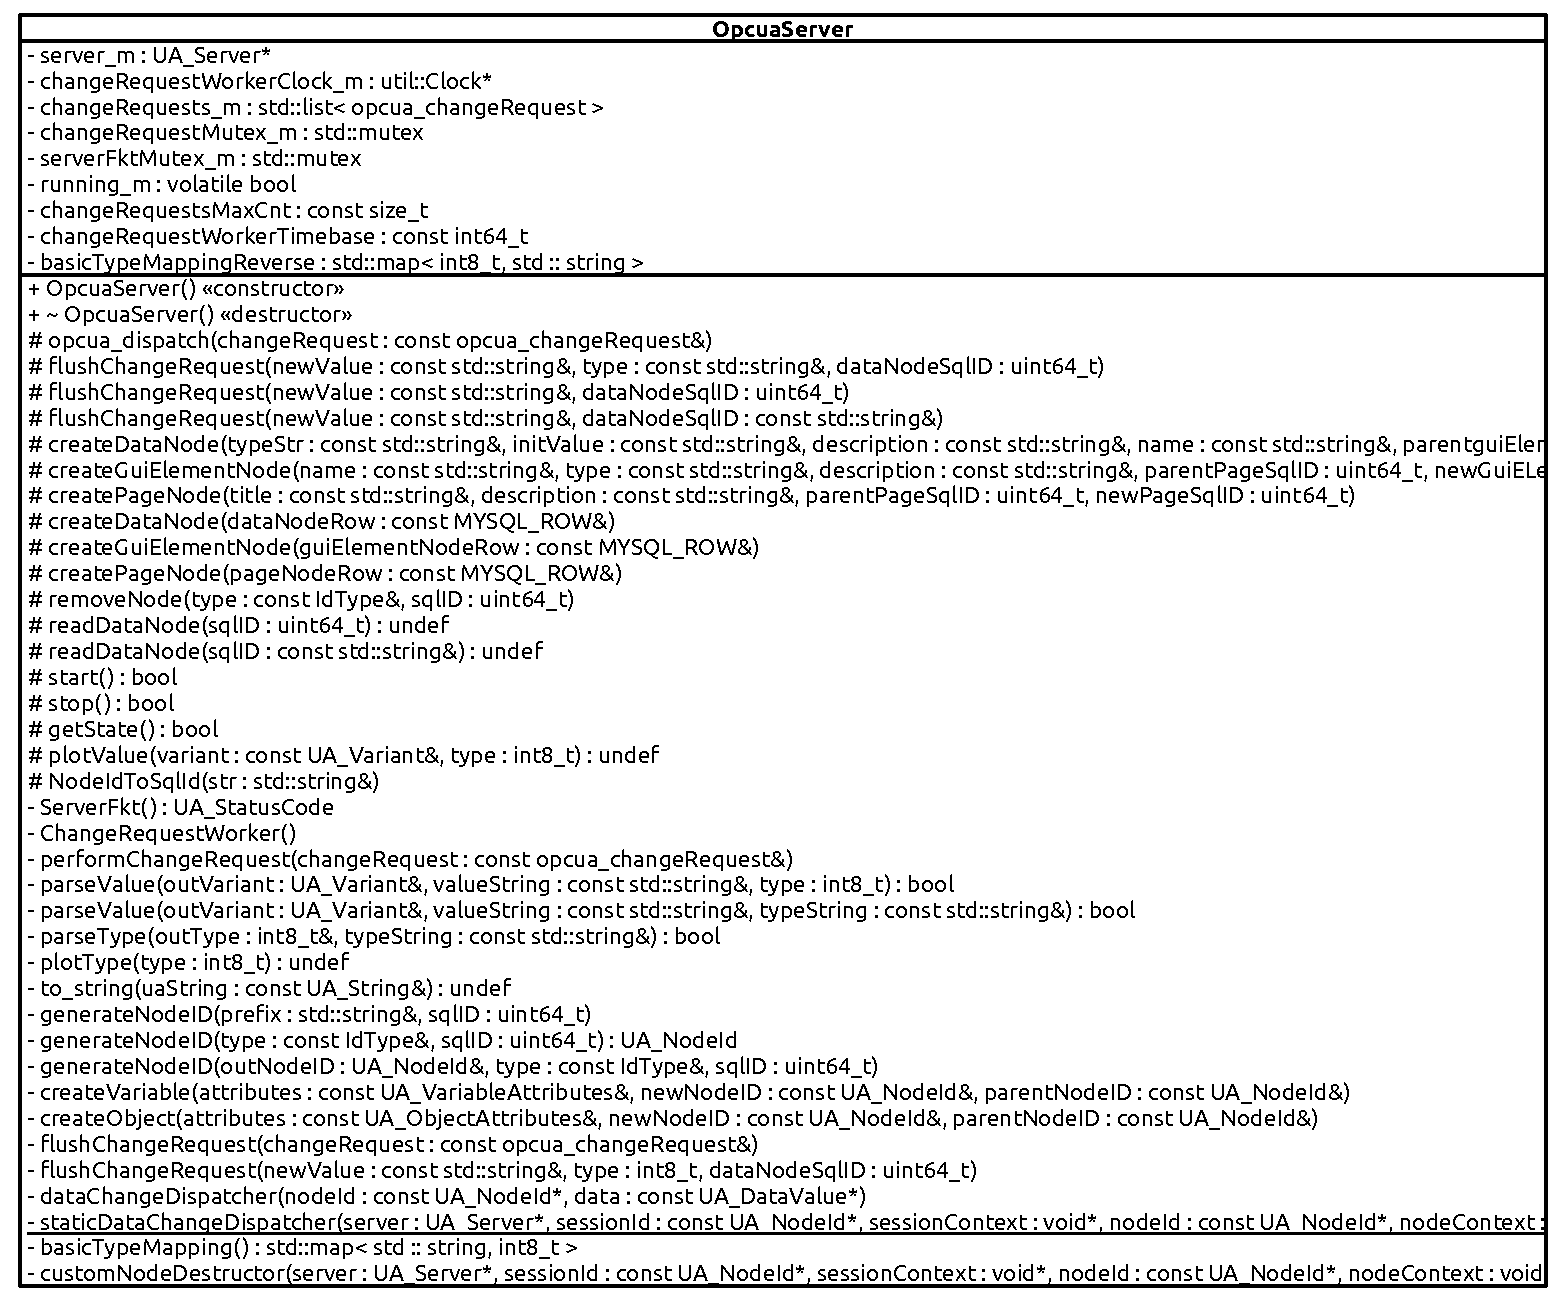
\includegraphics[width=\textwidth]{content/hauptteil/umsetzungPoC/backend/uml/classesOfOverview/OpcuaServer.pdf}
  \caption{Klassendiagramm der Klasse \eigenName{OpcuaServer}}
  \label{fig:backend:classDiag:OpcuaServer}
\end{figure}
Das Datenmodell des \ac{opcua} Servers beinhaltet nur die eingebauten Datentypen, also nur primitive Typen (Bool, String, Int \dots) und den Typ \emph{Object}.
Auf die Erstellung eines Datenmodells für jeden \emph{GuiElement} Typ wurde verzichtet, da diese an dieser Stelle nur zur Strukturierung der \emph{DataNodes} verwendet werden.
Die Datenstruktur, die den \acp{plc} zur Verfügung gestellt wird, enthält eine \emph{Page}, die wiederum eine \emph{Page} enthalten kann oder ein oder mehrere \emph{GuiElements}.
Jedes \emph{GuiElement} hat DataNodes deren Typ, entsprechend der Vorlage des \emph{GuiElement} Typs, in der \ac{sql} Datenbank festgelegt ist.
Die Übersetzung der Typen ist dabei durch das Attribut \eigenName{basicTypeMapping} definiert, das die in der Datenbank gespeicherten Typ Strings auf die eingebauten \ac{opcua} Datentypen mappt.
Die Umkehrung des Mappings ist in dem Attribut \mbox{\eigenName{basicTypeMappingReverse}} gespeichert.
Die Klasse \eigenName{OpcuaServer} stellt den anderen Klassen des Backends Methoden zur Verfügung, um \emph{DataNodes}, \emph{GuiElements} und \emph{Pages} auf dem OpcuaServer zu erstellen.
Die Methode \eigenName{readDataNode} ermöglicht das Auslesen einer einzelnen \emph{DataNode}. 
Sie wird verwendet, wenn eine Seite im Frontend neu geladen wird und noch keine Daten vorhanden sind.
Daten können entweder über die \ac{opcua} Schnittstelle geändert werden, oder durch eine Anforderung des Backends selbst.
Muss der Wert einer \emph{DataNode} geändert werden, so muss ein \eigenName{opcua\_changeRequest} Objekt erstellt werden (siehe Klassendiagramm in \refFig{fig:backend:classDiag:opcuaCR}), 
das die \eigenName{nodeID} und den neuen Wert der DataNode beinhaltet. Dieses Objekt wird anschließend an die Methode \eigenName{flushChangeRequest} übergeben.
\begin{figure}[ht]
  \centering
  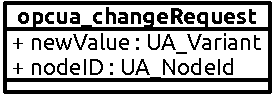
\includegraphics[width=0.2\textwidth]{content/hauptteil/umsetzungPoC/backend/uml/classesOfOverview/opcua_changeRequest.pdf}
  \caption{Klassendiagramm der Klasse \eigenName{opcua\_changeRequest}}
  \label{fig:backend:classDiag:opcuaCR}
\end{figure}
Das \eigenName{OpcuaServer} Objekt hat drei Threads. 
Ein Thread der exklusiv dem nativen Server der \emph{opne62541} Bibliothek zugeordnet ist und zwei Threads, mit denen zyklisch geprüft wird, 
ob \eigenName{opcua\_changeRequest} Objekte in der Warteschlange (Attribut \eigenName{changeRequests\_m}) vorhanden sind.
Sind in der Warteschlange \eigenName{opcua\_changeRequest} Objekte vorhanden, wird jedes Element an die Methode \eigenName{performChangeRequest} übergeben und aus der Warteschlange entfernt.
In der Methode \eigenName{performChangeRequest} wird dann die Änderung an der Datenstruktur durchgeführt. % eventuell noch den Trick mit NodeContext erklären () void*.....
Bei der Erstellung jeder \emph{DataNode} wird ein Handler angemeldet, der bei jedem Schreibvorgang auf die Node aufgerufen wird.
Dieser Handler ist als die Methode \eigenName{dataChangeDIspatcher} implementiert.
In diesem Handler wird verglichen, ob der Schreibvorgang ein Änderung des Werts darstellt. 
Ist das der Fall, wird die Methode \eigenName{opcua\_dispatch} mit einem \eigenName{opcua\_changeRequest} aufgerufen, der die \emph{NodeID} sowie den neuen Wert der \emph{DataNode} enthält.
Diese Methode wird schließlich in der \eigenName{Backend} Klasse reimplementiert und leitet die Änderung an die \eigenName{WebsocketServer} Klasse weiter. 